% Options for packages loaded elsewhere
\PassOptionsToPackage{unicode}{hyperref}
\PassOptionsToPackage{hyphens}{url}
%
\documentclass[
  ignorenonframetext,
]{beamer}
\usepackage{pgfpages}
\setbeamertemplate{caption}[numbered]
\setbeamertemplate{caption label separator}{: }
\setbeamercolor{caption name}{fg=normal text.fg}
\beamertemplatenavigationsymbolsempty
% Prevent slide breaks in the middle of a paragraph
\widowpenalties 1 10000
\raggedbottom
\setbeamertemplate{part page}{
  \centering
  \begin{beamercolorbox}[sep=16pt,center]{part title}
    \usebeamerfont{part title}\insertpart\par
  \end{beamercolorbox}
}
\setbeamertemplate{section page}{
  \centering
  \begin{beamercolorbox}[sep=12pt,center]{part title}
    \usebeamerfont{section title}\insertsection\par
  \end{beamercolorbox}
}
\setbeamertemplate{subsection page}{
  \centering
  \begin{beamercolorbox}[sep=8pt,center]{part title}
    \usebeamerfont{subsection title}\insertsubsection\par
  \end{beamercolorbox}
}
\AtBeginPart{
  \frame{\partpage}
}
\AtBeginSection{
  \ifbibliography
  \else
    \frame{\sectionpage}
  \fi
}
\AtBeginSubsection{
  \frame{\subsectionpage}
}
\usepackage{lmodern}
\usepackage{amssymb,amsmath}
\usepackage{ifxetex,ifluatex}
\ifnum 0\ifxetex 1\fi\ifluatex 1\fi=0 % if pdftex
  \usepackage[T1]{fontenc}
  \usepackage[utf8]{inputenc}
  \usepackage{textcomp} % provide euro and other symbols
\else % if luatex or xetex
  \usepackage{unicode-math}
  \defaultfontfeatures{Scale=MatchLowercase}
  \defaultfontfeatures[\rmfamily]{Ligatures=TeX,Scale=1}
\fi
\usetheme[]{CambridgeUS}
\usecolortheme{beaver}
% Use upquote if available, for straight quotes in verbatim environments
\IfFileExists{upquote.sty}{\usepackage{upquote}}{}
\IfFileExists{microtype.sty}{% use microtype if available
  \usepackage[]{microtype}
  \UseMicrotypeSet[protrusion]{basicmath} % disable protrusion for tt fonts
}{}
\makeatletter
\@ifundefined{KOMAClassName}{% if non-KOMA class
  \IfFileExists{parskip.sty}{%
    \usepackage{parskip}
  }{% else
    \setlength{\parindent}{0pt}
    \setlength{\parskip}{6pt plus 2pt minus 1pt}}
}{% if KOMA class
  \KOMAoptions{parskip=half}}
\makeatother
\usepackage{xcolor}
\IfFileExists{xurl.sty}{\usepackage{xurl}}{} % add URL line breaks if available
\IfFileExists{bookmark.sty}{\usepackage{bookmark}}{\usepackage{hyperref}}
\hypersetup{
  pdftitle={第十一章 时间序列分析方法},
  pdfauthor={授课教师:吴翔 ; wuhsiang@hust.edu.cn},
  hidelinks,
  pdfcreator={LaTeX via pandoc}}
\urlstyle{same} % disable monospaced font for URLs
\newif\ifbibliography
\usepackage{graphicx,grffile}
\makeatletter
\def\maxwidth{\ifdim\Gin@nat@width>\linewidth\linewidth\else\Gin@nat@width\fi}
\def\maxheight{\ifdim\Gin@nat@height>\textheight\textheight\else\Gin@nat@height\fi}
\makeatother
% Scale images if necessary, so that they will not overflow the page
% margins by default, and it is still possible to overwrite the defaults
% using explicit options in \includegraphics[width, height, ...]{}
\setkeys{Gin}{width=\maxwidth,height=\maxheight,keepaspectratio}
% Set default figure placement to htbp
\makeatletter
\def\fps@figure{htbp}
\makeatother
\setlength{\emergencystretch}{3em} % prevent overfull lines
\providecommand{\tightlist}{%
  \setlength{\itemsep}{0pt}\setlength{\parskip}{0pt}}
\setcounter{secnumdepth}{-\maxdimen} % remove section numbering
\usepackage{ctex}
\usepackage[fontsize=15pt]{scrextend}

\title{第十一章 时间序列分析方法}
\author{授课教师:吴翔 \newline \and \href{mailto:wuhsiang@hust.edu.cn}{\nolinkurl{wuhsiang@hust.edu.cn}}}
\date{OCT 15 - 18, 2019}

\begin{document}
\frame{\titlepage}

\begin{frame}
  \tableofcontents[hideallsubsections]
\end{frame}
\hypertarget{ux65f6ux95f4ux5e8fux5217ux5206ux6790ux6982ux8ff02ux4e2aux8bfeux65f6}{%
\section{时间序列分析概述(2个课时)}\label{ux65f6ux95f4ux5e8fux5217ux5206ux6790ux6982ux8ff02ux4e2aux8bfeux65f6}}

\begin{frame}{课程存储地址}
\protect\hypertarget{ux8bfeux7a0bux5b58ux50a8ux5730ux5740}{}

\begin{itemize}
\tightlist
\item
  课程存储地址: \url{https://github.com/wuhsiang/Courses}
\item
  资源:课件、案例数据及代码
\end{itemize}

\begin{figure}
\centering

\includegraphics[width=0.4\textwidth,height=\textheight]{../../QR.png}
\caption{课程存储地址}
\end{figure}

\end{frame}

\begin{frame}{参考教材}
\protect\hypertarget{ux53c2ux8003ux6559ux6750}{}

\begin{itemize}
\tightlist
\item
  Jonathan D. Cryer \& Kung-Sik Chan著,
  潘红宇等译.时间序列分析及应用(R语言)(原书第2版).
  北京:机械工业出版社. 2011.
\item
  James D. Hamilton著. 时间序列分析(2册). 北京:人民卫生出版社. 2015.
\item
  Robert I. Kabacoff著 . R语言实战(第二版). 北京:人民邮电出版社. 2016.
\end{itemize}

\end{frame}

\begin{frame}{本节知识点}
\protect\hypertarget{ux672cux8282ux77e5ux8bc6ux70b9}{}

\begin{itemize}
\tightlist
\item
  时间序列分析方法起源
\item
  时间序列基本概念
\item
  时间序列分析要素
\item
  时间序列分析建模
\end{itemize}

\end{frame}

\begin{frame}{11.1 时间序列分析方法起源}
\protect\hypertarget{ux65f6ux95f4ux5e8fux5217ux5206ux6790ux65b9ux6cd5ux8d77ux6e90}{}

英国洛桑试验站(Rothamsted Experimental Station,现为Rothamsted Research
洛桑研究所)

\end{frame}

\begin{frame}{Fisher与洛桑试验站}
\protect\hypertarget{fisherux4e0eux6d1bux6851ux8bd5ux9a8cux7ad9}{}

\end{frame}

\begin{frame}{洛桑试验站的小麦产量}
\protect\hypertarget{ux6d1bux6851ux8bd5ux9a8cux7ad9ux7684ux5c0fux9ea6ux4ea7ux91cf}{}

\begin{figure}
\centering
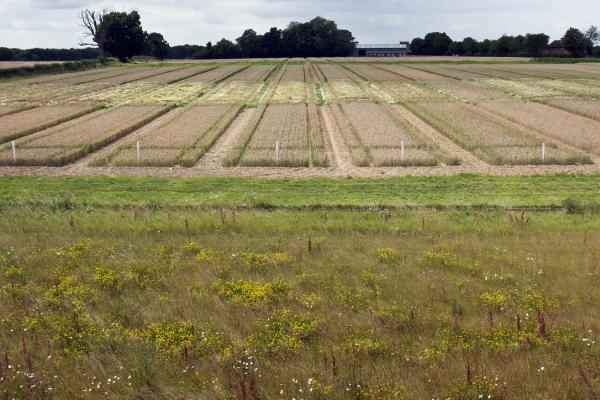
\includegraphics[width=0.55\textwidth,height=\textheight]{figures/rothamsted.jpg}
\caption{洛桑试验站}
\end{figure}

\end{frame}

\begin{frame}{如何预测小麦产量?}
\protect\hypertarget{ux5982ux4f55ux9884ux6d4bux5c0fux9ea6ux4ea7ux91cf}{}

\end{frame}

\begin{frame}{11.1.2 时间序列基本概念}
\protect\hypertarget{ux65f6ux95f4ux5e8fux5217ux57faux672cux6982ux5ff5}{}

\begin{itemize}
\tightlist
\item
  \textbf{时间序列(time series)}

  \begin{itemize}
  \tightlist
  \item
    定义:一组在特定时刻的观测值
  \item
    领域:广泛存在于宏观经济、金融财务以及医疗领域
  \end{itemize}
\item
  \textbf{时间序列分析(time series analysis)}

  \begin{itemize}
  \tightlist
  \item
    数据:时间序列数据(time series data),与横截面数据(cross
    sectional data)、面板数据(panel data),为三类主要的观测数据类型
  \item
    分析方法:通常基于宏观经济学理论建模,并采用宏观计量经济学方法分析
  \end{itemize}
\end{itemize}

\end{frame}

\begin{frame}{11.1.3 时间序列分析要素}
\protect\hypertarget{ux65f6ux95f4ux5e8fux5217ux5206ux6790ux8981ux7d20}{}

影响时间序列观测值的因素,可以分为以下几类:

\begin{enumerate}
\tightlist
\item
  趋势变动():
\item
  周期变动():
\item
  季节性变动():
\item
  不规则变动():
\end{enumerate}

通常将趋势和周期合并在一起考虑,成为趋势周期(trend-cycle),或简称趋势。

\end{frame}

\begin{frame}{11.1.4 时间序列建模}
\protect\hypertarget{ux65f6ux95f4ux5e8fux5217ux5efaux6a21}{}

时间序列 \[
Y_{t} = f(T_{t}, S_{t}, E_{t})
\]

\end{frame}

\begin{frame}{加法模型}
\protect\hypertarget{ux52a0ux6cd5ux6a21ux578b}{}

加法模型 \[
Y_{t} = T_{t} + S_{t} + E_{t}.
\]

\end{frame}

\begin{frame}{乘法模型}
\protect\hypertarget{ux4e58ux6cd5ux6a21ux578b}{}

乘法模型 \[
Y_{t} = T_{t} \times S_{t} \times E_{t}.
\]

\end{frame}

\hypertarget{ux65f6ux95f4ux5e8fux5217ux7ecfux5178ux5206ux6790ux65b9ux6cd53ux4e2aux8bfeux65f6}{%
\section{时间序列经典分析方法(3个课时)}\label{ux65f6ux95f4ux5e8fux5217ux7ecfux5178ux5206ux6790ux65b9ux6cd53ux4e2aux8bfeux65f6}}

\begin{frame}{本节知识点}
\protect\hypertarget{ux672cux8282ux77e5ux8bc6ux70b9-1}{}

\begin{itemize}
\tightlist
\item
  移动平均法
\item
  指数平滑法
\item
  生长曲线法
\item
  灰色系统预测法(略)
\end{itemize}

\end{frame}

\begin{frame}{11.2.1 移动平均法}
\protect\hypertarget{ux79fbux52a8ux5e73ux5747ux6cd5}{}

\begin{itemize}
\tightlist
\item
  简单移动平均法
\item
  加权移动平均法
\item
  趋势移动平均法
\end{itemize}

\end{frame}

\begin{frame}{简单移动平均法}
\protect\hypertarget{ux7b80ux5355ux79fbux52a8ux5e73ux5747ux6cd5}{}

\end{frame}

\begin{frame}{加权移动平均法}
\protect\hypertarget{ux52a0ux6743ux79fbux52a8ux5e73ux5747ux6cd5}{}

\end{frame}

\begin{frame}{趋势移动平均法}
\protect\hypertarget{ux8d8bux52bfux79fbux52a8ux5e73ux5747ux6cd5}{}

\end{frame}

\begin{frame}{11.2.2 指数平滑法}
\protect\hypertarget{ux6307ux6570ux5e73ux6ed1ux6cd5}{}

\begin{itemize}
\tightlist
\item
  一次指数平滑法
\item
  二次指数平滑法
\end{itemize}

\end{frame}

\begin{frame}{一次指数平滑法}
\protect\hypertarget{ux4e00ux6b21ux6307ux6570ux5e73ux6ed1ux6cd5}{}

\end{frame}

\begin{frame}{二次指数平滑法}
\protect\hypertarget{ux4e8cux6b21ux6307ux6570ux5e73ux6ed1ux6cd5}{}

\end{frame}

\begin{frame}{11.2.3 生长曲线法}
\protect\hypertarget{ux751fux957fux66f2ux7ebfux6cd5}{}

\begin{itemize}
\tightlist
\item
  指数曲线模型
\item
  Logistic曲线模型
\end{itemize}

\end{frame}

\begin{frame}{指数曲线模型}
\protect\hypertarget{ux6307ux6570ux66f2ux7ebfux6a21ux578b}{}

\end{frame}

\begin{frame}{Logistic曲线模型}
\protect\hypertarget{logisticux66f2ux7ebfux6a21ux578b}{}

\end{frame}

\hypertarget{ux65f6ux95f4ux5e8fux5217ux6848ux4f8bux5206ux67901ux4e2aux8bfeux65f6}{%
\section{时间序列案例分析(1个课时)}\label{ux65f6ux95f4ux5e8fux5217ux6848ux4f8bux5206ux67901ux4e2aux8bfeux65f6}}

\begin{frame}{本节知识点}
\protect\hypertarget{ux672cux8282ux77e5ux8bc6ux70b9-2}{}

\begin{itemize}
\item
  时间序列分析建模与预测
\item
  \url{https://github.com/wuhsiang/Courses/blob/master/healthinfo/cases/case-dhaka.Rmd})
\end{itemize}

\end{frame}

\hypertarget{ux65f6ux95f4ux5e8fux5217ux5206ux6790ux5b9eux4e602ux4e2aux8bfeux65f6}{%
\section{时间序列分析实习(2个课时)}\label{ux65f6ux95f4ux5e8fux5217ux5206ux6790ux5b9eux4e602ux4e2aux8bfeux65f6}}

\end{document}
